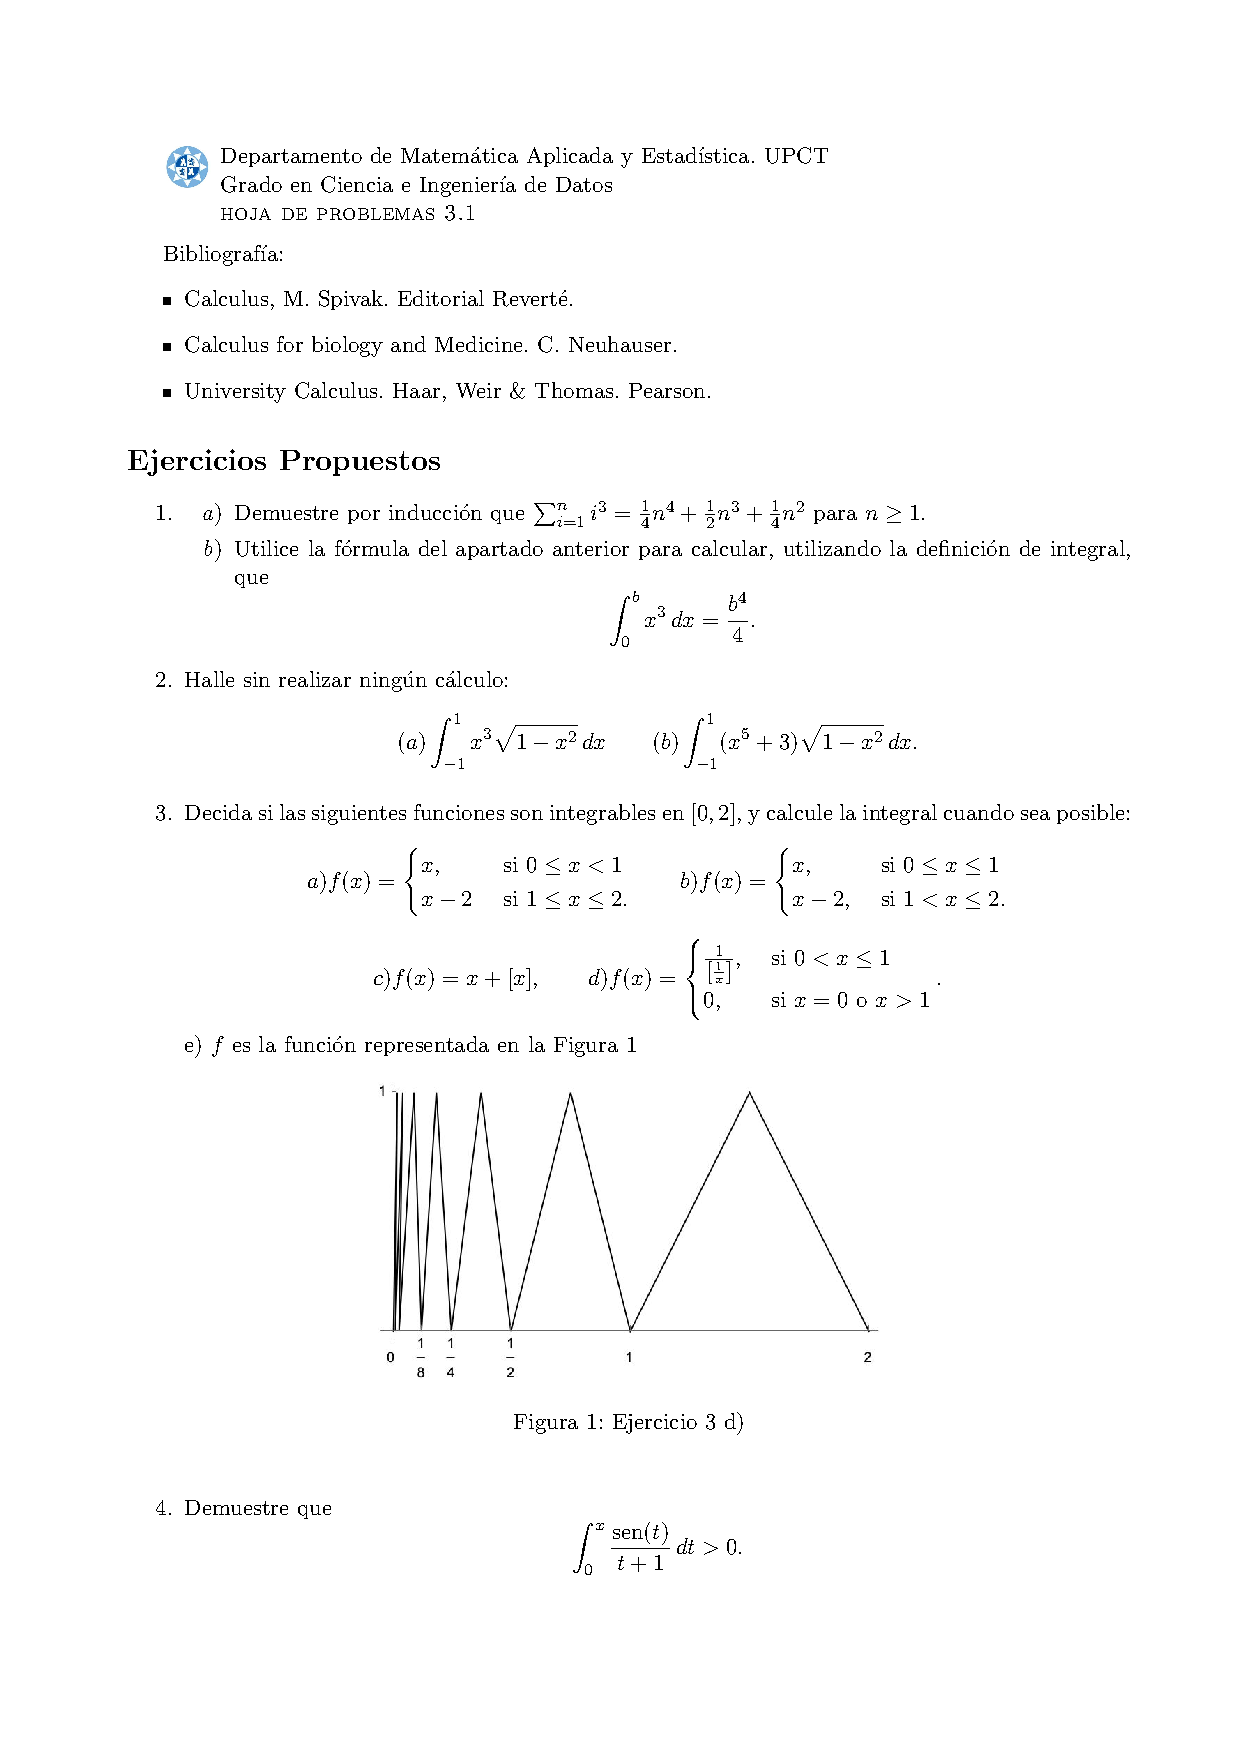
\includepdf[pages=-]{Tareas/Tema 3/Hoja 3.1/Hoja 3.1.pdf}

\begin{enumerate}[label=\color{red}\textbf{\arabic*)}, leftmargin=*]
	\item \begin{enumerate}[label=\color{red}\alph*)]
		\item \lb{Demuestre por inducción que $\sum_{i=1}^{n}i^3=\dfrac{1}{4}n^4+\dfrac{1}{2}n^3+\dfrac{1}{4}n^2$ para $n\ge1$.}
		\item \lb{Utilice la fórmula del apartado anterior para calcular, utilizando la definición de integral, que \[ \int_{0}^{b}x^3\dx=\dfrac{b^4}{4}. \]}
	\end{enumerate}
	\item \lb{Halle sin realizar ningún cálculo:}
	\begin{enumerate}[label=\color{red}\alph*)]
		\item $\db{\int_{-1}^{1}x^3\sqrt{1-x^2}\dx=}$
		\item $\db{\int_{-1}^{1}(x^5+3)\sqrt{1-x^2}\dx}$
	\end{enumerate}
	\item \lb{Decida si las siguientes funciones son integrables en $[0,2]$, y calcule la integral cuando sea posible:}
	\begin{enumerate}[label=\color{red}\alph*)]
		\item $\db{f(x)=\begin{cases}
				x & \text{si }0\le x<1\\
				x-2 & \text{si }1\le x\le2
		\end{cases}}$
	
	$\int_0^1x\dx+\int_1^2x-2\dx=0$
	
	\begin{tikzpicture}[scale=2]
		
		
		\fill[lightblue] (1,-1) circle (1.5pt);
		\draw[lightblue] (0,0) -- (1,1);
		\draw[lightblue] (1,-1) -- (2,0);
		
            \fill[lightblue!10] (0,0) -- (1,1) |- (0,0);
            \fill[lightblue!10] (2,0) -- (1,-1) |- (2,0);
            \draw[lightblue,dashed] (1,1) -- (1,-1);
            \draw[lightblue, line width=1.5pt] (1,1) circle (1.5pt);
            \draw (-1,0) -- (2.2,0);
            \draw (0,-1) -- (0,1.2);
	\end{tikzpicture}
	\item $\db{f(x)=\begin{cases}
			x & \text{si }0\le x\le1\\
			x-2 & \text{si }1<x\le2
	\end{cases}}$

$\int_{0}^{2}f(x)\dx=0$

\begin{tikzpicture}[scale=2]
	
	\fill[lightblue!10] (0,0) -- (1,1) |- (0,0);
	\fill[lightblue!10] (2,0) -- (1,-1) |- (2,0);
	\fill[lightblue] (1,1) circle (1.5pt);
	\draw[lightblue, line width=1.5pt] (1,-1) circle (1.5pt);
	\draw[lightblue] (0,0) -- (1,1);
	\draw[lightblue] (1,-1) -- (2,0);
	\draw[lightblue,dashed] (1,1) -- (1,-1);
      \draw (-1,0) -- (2.2,0);
      \draw (0,-1) -- (0,1.2);
\end{tikzpicture}
\item $\db{f(x)=x+[x]}\longrightarrow f(x)=\begin{cases}
	x & 0<x<1\\
	x+1 & 1\le x\le 2\\
	4 & x=2
\end{cases}\qquad\int_{0}^{2}x+[x]\dx=3$

\begin{center}
	\begin{tikzpicture}[scale=1.5, baseline=(current bounding box.center)]
		\draw (-1,0) -- (3.5,0);
		\draw (0,-1) -- (0,2.5);
		\draw[lightblue] (1,1) -- (2,1);
            \draw[lightblue]  (2,2) -- (3,2);
		\fill[lightblue] (1,1) circle (1.5pt);
		\fill[lightblue] (2,2) circle (1.5pt);
		\foreach \x in {1,2,3}{
		\node[below] at (\x,0) {\x};
		};
		\draw[lightblue,dashed] (2,2) -- (2,0);
            \draw[lightblue,dashed] (1,0) -- (1,1);
	\end{tikzpicture}\qquad
	\begin{tikzpicture}[scale=1.5, baseline=(current bounding box.center)]
            \fill[fill=lightblue!10] (0,0) -- (1,1) |- (0,0);
            \fill[fill=lightblue!10] (1,2) -- (2,3) |- (1,2);
		\draw (-1,0) -- (2.5,0);
		\draw (0,-1) -- (0,4);
		\draw[lightblue, line width=1.5pt] (1,1) circle (1.5pt);
		\fill[lightblue] (1,2) circle (1.5pt);
		\draw[lightblue] (0,0) -- (1,1); 
            \draw[lightblue] (1,2) -- (2,3) ;
		\draw[lightblue,dashed] (1,1) -- (1,0);
		\draw[lightblue,dashed] (1,2) -- (2,2) ;
		\draw[lightblue,dashed] (2,3) -- (2,0);
	\end{tikzpicture}
\end{center}
\item $\db{f(x)=\begin{cases}
		\dfrac{1}{\left[\frac{1}{x}\right]} & \text{si }<x\le1\\
		0 & \text{si }x=0\text{ o }x>1
\end{cases}}$

$\begin{array}{l}
      \left(1-\dfrac{1}{2}\right)\cdot1+\left(\dfrac{1}{2}-\dfrac{1}{3}\right)\cdot\dfrac{1}{2}+\left(\dfrac{1}{3}-\dfrac{1}{4}\right)\cdot\dfrac{1}{3}+\cdots+\left(\dfrac{1}{n}-\dfrac{1}{n-1}\right)\cdot\dfrac{1}{n}\\
      \begin{aligned}
	\int_{0}^{2}f(x)\dx&=\int_{0}^{1}f(x)\dx+\int_{1}^{2}f(x)\dx\\
	&=\sum_{n=1}^{\infty}\left(\dfrac{1}{n}-\dfrac{1}{n+1}\right)\cdot\dfrac{1}{n}\\
	&=\sum_{n=1}^{\infty}\dfrac{1}{n^2}-\dfrac{1}{n\cdot(n+1)}\\
      &=\sum_{n=1}^{\infty}\dfrac{1}{n^2}-\sum_{n=1}^{\infty}\dfrac{1}{n(n+1)}=\dfrac{\pi^2}{6}-1
\end{aligned}\\
\dfrac{1}{n(n+1)}=\dfrac{1}{n}+\dfrac{-1}{n+1}=\dfrac{A(n+1)Bn}{n(n+1)}\\
1 = An+Bn+A\longrightarrow A+B=0\\
A=1\longrightarrow B=-1\\
\mathcal{S}_m=\sum_{n=1}^{m}\dfrac{1}{n}-\dfrac{1}{n+1}=\bboxed{1}-\cancel{\dfrac{1}{2}}+\cancel{\dfrac{1}{2}}-\cancel{\dfrac{1}{3}}+\cancel{\dfrac{1}{3}}-\cancel{\dfrac{1}{4}}+\cdots+\cancel{\dfrac{1}{m}}\bboxed{-\dfrac{1}{m+1}}
\end{array}$

\item \db{$f$ es la función representada en la Figura 1}

\begin{figure}[h]
	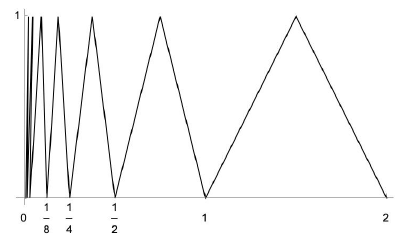
\includegraphics{"Tareas/Tema 3/Hoja 3.1/Figura 1.png"}
	\centering
	\caption*{\db{Figura 1: Ejercicio 3 d)}}
\end{figure}

$\begin{aligned}
	\int_{0}^{2}f(x)\dx&=1\cdot\dfrac{1}{2}+\dfrac{1}{2}\cdot\dfrac{1}{2}+\dfrac{1}{2^2}\cdot\dfrac{1}{2}+\cdots+\dfrac{1}{2^n}\cdot\dfrac{1}{2}\\
&=\dfrac{1}{2}+\dfrac{1}{2^2}+\dfrac{1}{2^3}+\cdots+\dfrac{1}{2^n}\\
&=\sum_{n=1}^{\infty}\dfrac{1}{2^n}=\dfrac{\frac{1}{2}}{1-\frac{1}{2}}=\dfrac{\frac{1}{2}}{\frac{1}{2}}=\bboxed{1}
\end{aligned}$
	\end{enumerate}
\item \lb{Demuestre que \[ \int_{0}^{x}\dfrac{\sin(t)}{t+1}\dt>0. \]}

$x>0$

\begin{tikzpicture}% function
	\begin{axis}[xlabel=x,ylabel=y,axis lines=center,
            xtick={-2*pi, -3*pi/2, -pi, -pi/2, 0, pi/2, pi, 3*pi/2, 2*pi}, 
            xticklabels={$-2\pi$, $-\frac{3\pi}{2}$, $-\pi$, $-\frac{\pi}{2}$, $0$, $\frac{\pi}{2}$, $\pi$, $\frac{3\pi}{2}$, $2\pi$},
            ]
		\addplot[lightblue, fill=lightblue!10,domain=0:4*pi, samples=150] {sin(deg(x))/(x+1)};
	\end{axis}
\end{tikzpicture}

$\begin{array}{l}
\int_{0}^{x}\dfrac{\sin(t)}{t+1}\dt=\int_{0}^{\pi}\dfrac{\sin(t)}{t+1}\dt+\lbb{\int_{\pi}^{2\pi}\dfrac{\sin(t)}{t+1}\dt}{(\ast)}+\cdots+\int_{(n-1)\pi}^{x}\dfrac{\sin(t)}{t+1}\dt+\int_{0}^{\pi}\dfrac{\sin(t)}{t+1}\dt>\int_{0}^{\pi}\dfrac{\sin(t)}{\pi+t+1}\dt\\
\lb{(\ast)=}\left\{\begin{array}{l|l}
      u=t-\pi & t=u+\pi\\
      \du=\dt
\end{array}\right\}=-\int_{0}^{\pi}\dfrac{\sin(u)}{u+\pi+1}\du
\end{array}$
\item \lb{Demuestre que \[ \int_{ca}^{cb}f(t)\dt=x\int_{a}^{b}f(ct)\dt. \]}
$\begin{array}{l}
      \int_{ca}^{cb}f(t)\dt=\int_a^bf(cs)\cdot c\mathrm{d}s=c\int_{a}^{b}f(c\cdot s)\mathrm{d}s\\
      \begin{array}{ll}
            t=c\cdot s & \lb{ca\longrightarrow=c\cdot} s\longrightarrow s=a\\
            \dt=c\cdot \mathrm{d}s & \lb{cb\longrightarrow c\cdot b=c\cdot s\longrightarrow s=b}
      \end{array}
\end{array}$
\item \lb{Sabiendo }
\begin{enumerate}[label=\color{red}\alph*)]
      \item $\db{\int_{0}^{\infty}=x^2e^{-x^2}\dx}$
      
      \db{Observación: Integra por partes. $u=x,\dv=xe^{-x^2}\dx$. La función $f(x)=e^{-x^2}$ es par.}
      \item $\db{\int_{-\infty}^{\infty}=e^{\frac{(x-\mu)^2}{2\sigma^2}}\dx}$
      
      \db{Observación: Haz el cambio de variable $t=\dfrac{x-\mu}{\sqrt{2}\sigma}$.}
      \item $\db{\int_{0}^{\infty}\dfrac{e^{-x}}{\sqrt{x}}\dx}$
      
      \db{Observación: Haz el cambio de variable $t=\sqrt{x}$.}
\end{enumerate}
\item \lb{Se define la funcion $\Gamma(\alpha)=\int_{0}^{\infty}e^{-x}x^{\alpha-1}\dx$, si $\alpha>0$.}
\begin{enumerate}[label=\color{red}\alph*)]
      \item \db{Justifique la covergencia de la integral cuando $\alpha>0$.}
      
      \begin{itemize}
            \item $\alpha>1\qquad\int_{0}^{\infty}e^{-x}\cdot x^{\alpha-1}\quad \int_{0}^{\infty}e^{-\frac{x}{2}}\dx$
            
            $\begin{array}{l}
                  0<\alpha<1\\
                  0<x<1
            \end{array}\qquad e^{-x}\cdot x^{\alpha-1}=\dfrac{e^{-x}}{x^{1-\alpha}}\le\dfrac{1}{x^{1-\alpha}}$
            \item $0<\alpha<1\qquad\int_{0}^{1}e^{-x}x^{\alpha-1}\dx+\int_{1}^{+\infty}e^{-x}\cdot x^{\alpha-1}\dx$
            
            $\begin{array}{l}
                  0<\alpha<1\\
                  1<x<\infty
            \end{array}\qquad \begin{array}{l}
            e^{-x}\cdot x^{\alpha-1}=\dfrac{e^{-x}}{x^{1-\alpha}}\le e^{-x}\quad \int_{1}^{\infty}e^{-x}\dx=\lim_{n\to\infty}\left[-e^{-x}\right]_0^b=\bboxed{1}\\
            g(x)=x^{\alpha-1}\xrightarrow{\alpha=\frac{1}{2}}x^{-\frac{1}{2}}=\dfrac{1}{\sqrt{x}}\\
            g'(x)=(x-1)\cdot x^{\alpha-2}
            \end{array}$
      \end{itemize}
      \item \db{Demuestre (integrando por partes) que $\Gamma(\alpha+1)=\alpha\Gamma(\alpha)$, para todo $\alpha>0$. Deduzca utilizando inducción, que $\Gamma(n+1)=n!$.}
      \item \db{Calcule en términos de la función $\Gamma(\alpha)$:}
      \begin{enumerate}[label=\color{blue}\alph*)]
            \item $\int_{0}^{\infty}e^{\sqrt[3]{x}}\dx$
            \item $\int_{0}^{\infty}x^ne^{-\frac{x^2}{2}}\dx,\quad n\in\N$
      \end{enumerate}
\end{enumerate}
\item \lb{Halle las derivadas de cada una de las siguientes funciones:}
\begin{enumerate}[label=\color{red}\alph*)]
	\item $\db{F(x)=\int_{a}^{x^3}\sin^3(t)\dt}$
	
	$\begin{array}{l}
		F'(x)=G'(x^3)\cdot 3x^2=\sin^3(x^3)\cdot3\cdot x^2\\
		\boxed{G(x)=\int_{a}^{x}\sin^3(t)\dt}\longrightarrow \text{T.F.I (Teorema Fundamental de la Integral)}\\
		G'(x)=\sin^3(x)
	\end{array}$
	\item $\db{F(x)=\int_{y}^{\left(\int_{1}^{x}\sin^3(t)\dt\right)}\dfrac{1}{1+\sin^6(t)+t^2}\dt}$
	
	$\begin{array}{l}
		g(x)=\int_{1}^{1}\sin^3(t)\dt\qquad g'(x)=\sin^3(x)\qquad F'(x)=G'(g(x))\cdot g'(x)=\dfrac{\sin^3(x)}{1+\sin^6\left(g(x)\right)+g(x)^2}\\
		G(x)=\int_{x}^{y}\dfrac{1}{1+\sin^6(t)+t^2}\longrightarrow G'(x)=\dfrac{1}{1+\sin^6(t)+x^2}\\
		y\in\mathbb{R}
	\end{array}$
	\item $\db{F(x)=\int_{a}^{b}\dfrac{x}{1+t^2+\sin^2t}\dt}$
	\item \db{Halle $(F^{-1})'(x)$ en términos de $F^{-1}(x)$ siendo $F(x)=\int_{1}^{x}\dfrac{1}{t}\dt$.}
\end{enumerate}
\item \lb{Halle $F'(x)$ si $F(x)=\int_{0}^{x}x\:f(t)\dt$.}
\item \lb{Si $f$ es continua en $[0,1]$, calcule $\lim_{x\to0^+}x\int_{x}^{1}\dfrac{f(t)}{t}\dt$.}
\item \lb{Utilice el criterio de comparación para determinar si las integrales siguientes convergen:}
\begin{enumerate}[label=\color{red}\alph*)]
	\item $\db{\int_{\pi}^{\infty}\dfrac{\sin^2(2x)}{x^2}\dx}$
	\item $\db{\int_{1}^{\infty}\dfrac{x}{\sqrt{1+x^5}}\dx}$
\end{enumerate}
\item \lb{Sea $f(x)=x^n$, siendo $n$ un entero positivo. Determinar el valor medio de $f$ en el intervalo $[a,b]$.}
\end{enumerate}